\chapter{LOSS FUNCTION INVESTIGATION FOR MYOCARDIUM SEGMENTATION} 
 
\section{Overview}
\label{sec:ch5-intro-overview}  


This chapter presents the second stage of the proposed deep learning framework for myocardial infarction assessment by investigating the influence of different loss functions on myocardium segmentation performance. Building upon the cardiac structure segmentation framework established in Chapter IV, this study aims to identify a loss function that produces a more accurate and reliable anatomical myocardium representation for subsequent myocardial scar segmentation and quantitative scar assessment.  

The previous chapter established an enhanced U-Net framework incorporating fuzzy pooling for cardiac structure segmentation, demonstrating its capability to accurately segment the left ventricle (LV), right ventricle (RV), and myocardium (MYO). The enhanced segmentation backbone adopted in this chapter follows the architecture previously developed in the first stage of this research while maintaining identical preprocessing procedures and training configurations. Although satisfactory segmentation performance was achieved, network architecture alone does not completely determine segmentation quality. During model training, the loss function defines how prediction errors are quantified and guides parameter updates throughout the learning process. Consequently, different loss functions may produce substantially different segmentation characteristics even when an identical network architecture is applied \citep{Ronneberger2015,Jadon2020,Ma2021}. Furthermore, previous work demonstrated that incorporating fuzzy pooling improves feature preservation during down-sampling, providing a suitable segmentation backbone for investigating different optimization objectives \citep{Riandini2023MeMeA}. 

Among the three cardiac structures investigated in Chapter IV, the myocardium represents the most challenging segmentation target. Unlike the relatively homogeneous regions of the left and right ventricles, the myocardium forms a thin ring-shaped anatomical structure with complex boundaries and occupies only a small proportion of the entire cardiac MR image. These characteristics create a pronounced imbalance between foreground and background pixels while simultaneously increasing the difficulty of preserving continuous myocardial contours. As a result, segmentation models trained using conventional pixel-wise loss functions may achieve satisfactory global overlap measurements while still producing suboptimal segmentation of myocardial boundaries, thereby affecting the reliability of subsequent quantitative cardiac analysis and pathology assessment \citep{Milletari2016,Lin2017,Berman2018,Karimi2019,Ma2021}.

Motivated by these challenges, this chapter investigates how different loss functions influence myocardium segmentation performance while maintaining an identical segmentation framework. Five representative loss functions are systematically evaluated, comprising four established loss functions, namely Cross-Entropy, Dice Loss, Focal Loss, and Lovász-Softmax, together with the proposed CrossLov loss. The enhanced U-Net architecture with fuzzy pooling developed in Chapter IV is retained without modification throughout all experiments. Consequently, the experimental design isolates the influence of individual loss functions on myocardium segmentation performance from architectural and implementation factors, allowing performance differences to be attributed solely to the learning characteristics of each investigated loss function \citep{Riandini2025Array}. 

The comparative investigation is conducted from complementary perspectives to provide a comprehensive understanding of the characteristics of each investigated loss function. During the training process, convergence behaviour is analysed through the evolution of training loss, Dice score, computational time, and the best-performing epoch. The resulting segmentation performance is subsequently evaluated quantitatively using the Dice Similarity Coefficient (DSC), Intersection over Union (IoU), and Hausdorff Distance (HD), followed by qualitative visual assessment of myocardial boundary preservation. This integrated evaluation provides complementary information regarding segmentation performance by combining overlap-based measurements, distance-based evaluation, and qualitative visual assessment \citep{Taha2015,Jadon2020,Riandini2025Array}.  

The comparative investigation is conducted from complementary perspectives to provide a comprehensive understanding of the characteristics of each investigated loss function. During the training process, convergence behaviour is analysed through the evolution of training loss, Dice Score, computational time, and the best-performing epoch. The resulting segmentation performance is subsequently evaluated quantitatively using the Dice Similarity Coefficient (DSC), Intersection over Union (IoU), and Hausdorff Distance (HD), followed by qualitative visual assessment of myocardial boundary preservation. This integrated evaluation combines optimization behaviour, overlap-based measurements, distance-based evaluation, and qualitative visual assessment to provide complementary evidence regarding the effectiveness of each investigated loss function \citep{Taha2015,Jadon2020,Ma2021,Riandini2025Array}.

Unlike many segmentation studies that simultaneously modify both the network architecture and the optimization strategy, this study intentionally fixes the segmentation backbone while varying only the loss function. Such a controlled experimental design enables a fair comparison in which differences in segmentation performance can be directly attributed to the optimization objective rather than architectural complexity. Consequently, the findings provide a comprehensive understanding of the complementary strengths and limitations of pixel-wise, region-based, and hybrid learning objectives for myocardium segmentation under an identical segmentation framework \citep{Riandini2025Array}.

The primary contribution of this chapter is to identify an effective loss function for reliable myocardium segmentation using a fixed enhanced U-Net framework with fuzzy pooling. Rather than introducing a new segmentation architecture, this study provides a comprehensive understanding of how different learning objectives influence myocardium segmentation performance and identifies the most suitable loss function for accurate and reliable myocardium segmentation under a fixed segmentation method. The findings presented in this chapter establish a more reliable myocardium representation that supports the residual attention-based myocardial scar assessment framework presented in Chapter VI. 

\section{Myocardium Segmentation Framework}
\label{sec:ch5-framework} 

\subsection{Framework Overview}
\label{subsec:ch5-overview}  

Building upon the enhanced U-Net framework with fuzzy pooling established in Chapter IV, this chapter investigates the influence of different loss functions on myocardium segmentation while maintaining an identical segmentation architecture. Rather than proposing a new segmentation network, the enhanced U-Net with fuzzy pooling developed in the previous chapter is retained as a fixed segmentation backbone throughout this study. Consequently, the selected loss function becomes the sole independent experimental variable, enabling the influence of different optimization objectives on myocardium segmentation performance to be investigated without interference from architectural modifications, preprocessing procedures, or training configurations.   

Unlike Chapter IV, which addressed the simultaneous segmentation of the left ventricle (LV), right ventricle (RV), and myocardium (MYO), the present study focuses exclusively on myocardium ring segmentation. This narrower scope is motivated by the anatomical characteristics of the myocardium, which forms a thin ring-shaped structure with complex geometry, indistinct boundaries, and relatively small spatial occupancy within cardiac MR images. These characteristics create a pronounced foreground-background class imbalance while simultaneously increasing the difficulty of preserving continuous myocardial contours. Consequently, myocardium segmentation requires learning objectives capable of improving both regional overlap and boundary consistency to achieve anatomically reliable segmentation results \citep{Milletari2016,Berman2018,Karimi2019,Ma2021}

The overall experimental workflow adopted in this chapter is illustrated in Figure~\ref{fig:ch5-framework}. The workflow begins with cine cardiac MR images acquired from the ACDC dataset, followed by image preprocessing before being provided as input to the enhanced U-Net incorporating fuzzy pooling. During network training, five representative loss functions, namely Cross-Entropy, Dice Loss, Focal Loss, Lovász-Softmax, and the proposed CrossLov loss, are independently incorporated into the optimization process. Throughout all experiments, the network architecture, dataset partition, optimizer, hyperparameter settings, and evaluation protocol are maintained without modification, ensuring that the investigated loss function constitutes the only independent experimental variable. This controlled experimental design enables a fair comparison in which the observed performance differences can be attributed solely to the learning characteristics of each investigated loss function rather than to variations in network architecture or implementation \citep{Riandini2025Array}. 

Following model training, the resulting myocardium segmentation masks are evaluated through complementary quantitative and qualitative analyses. Training behaviour is first examined using convergence characteristics, training loss, Dice Score, computational time, and the best-performing epoch achieved by each investigated loss function. The segmentation results are subsequently evaluated using the Dice Similarity Coefficient (DSC), Intersection over Union (IoU), and Hausdorff Distance (HD), followed by qualitative visual comparison of representative myocardium segmentation results. Collectively, these complementary evaluations provide a comprehensive understanding of how different optimization objectives influence myocardium segmentation performance and facilitate the identification of the most appropriate loss function for accurate and reliable myocardium segmentation under a fixed segmentation framework \citep{Taha2015,Jadon2020,Ma2021,Riandini2025Array}.

\begin{figure}[htbp]
	\centering
	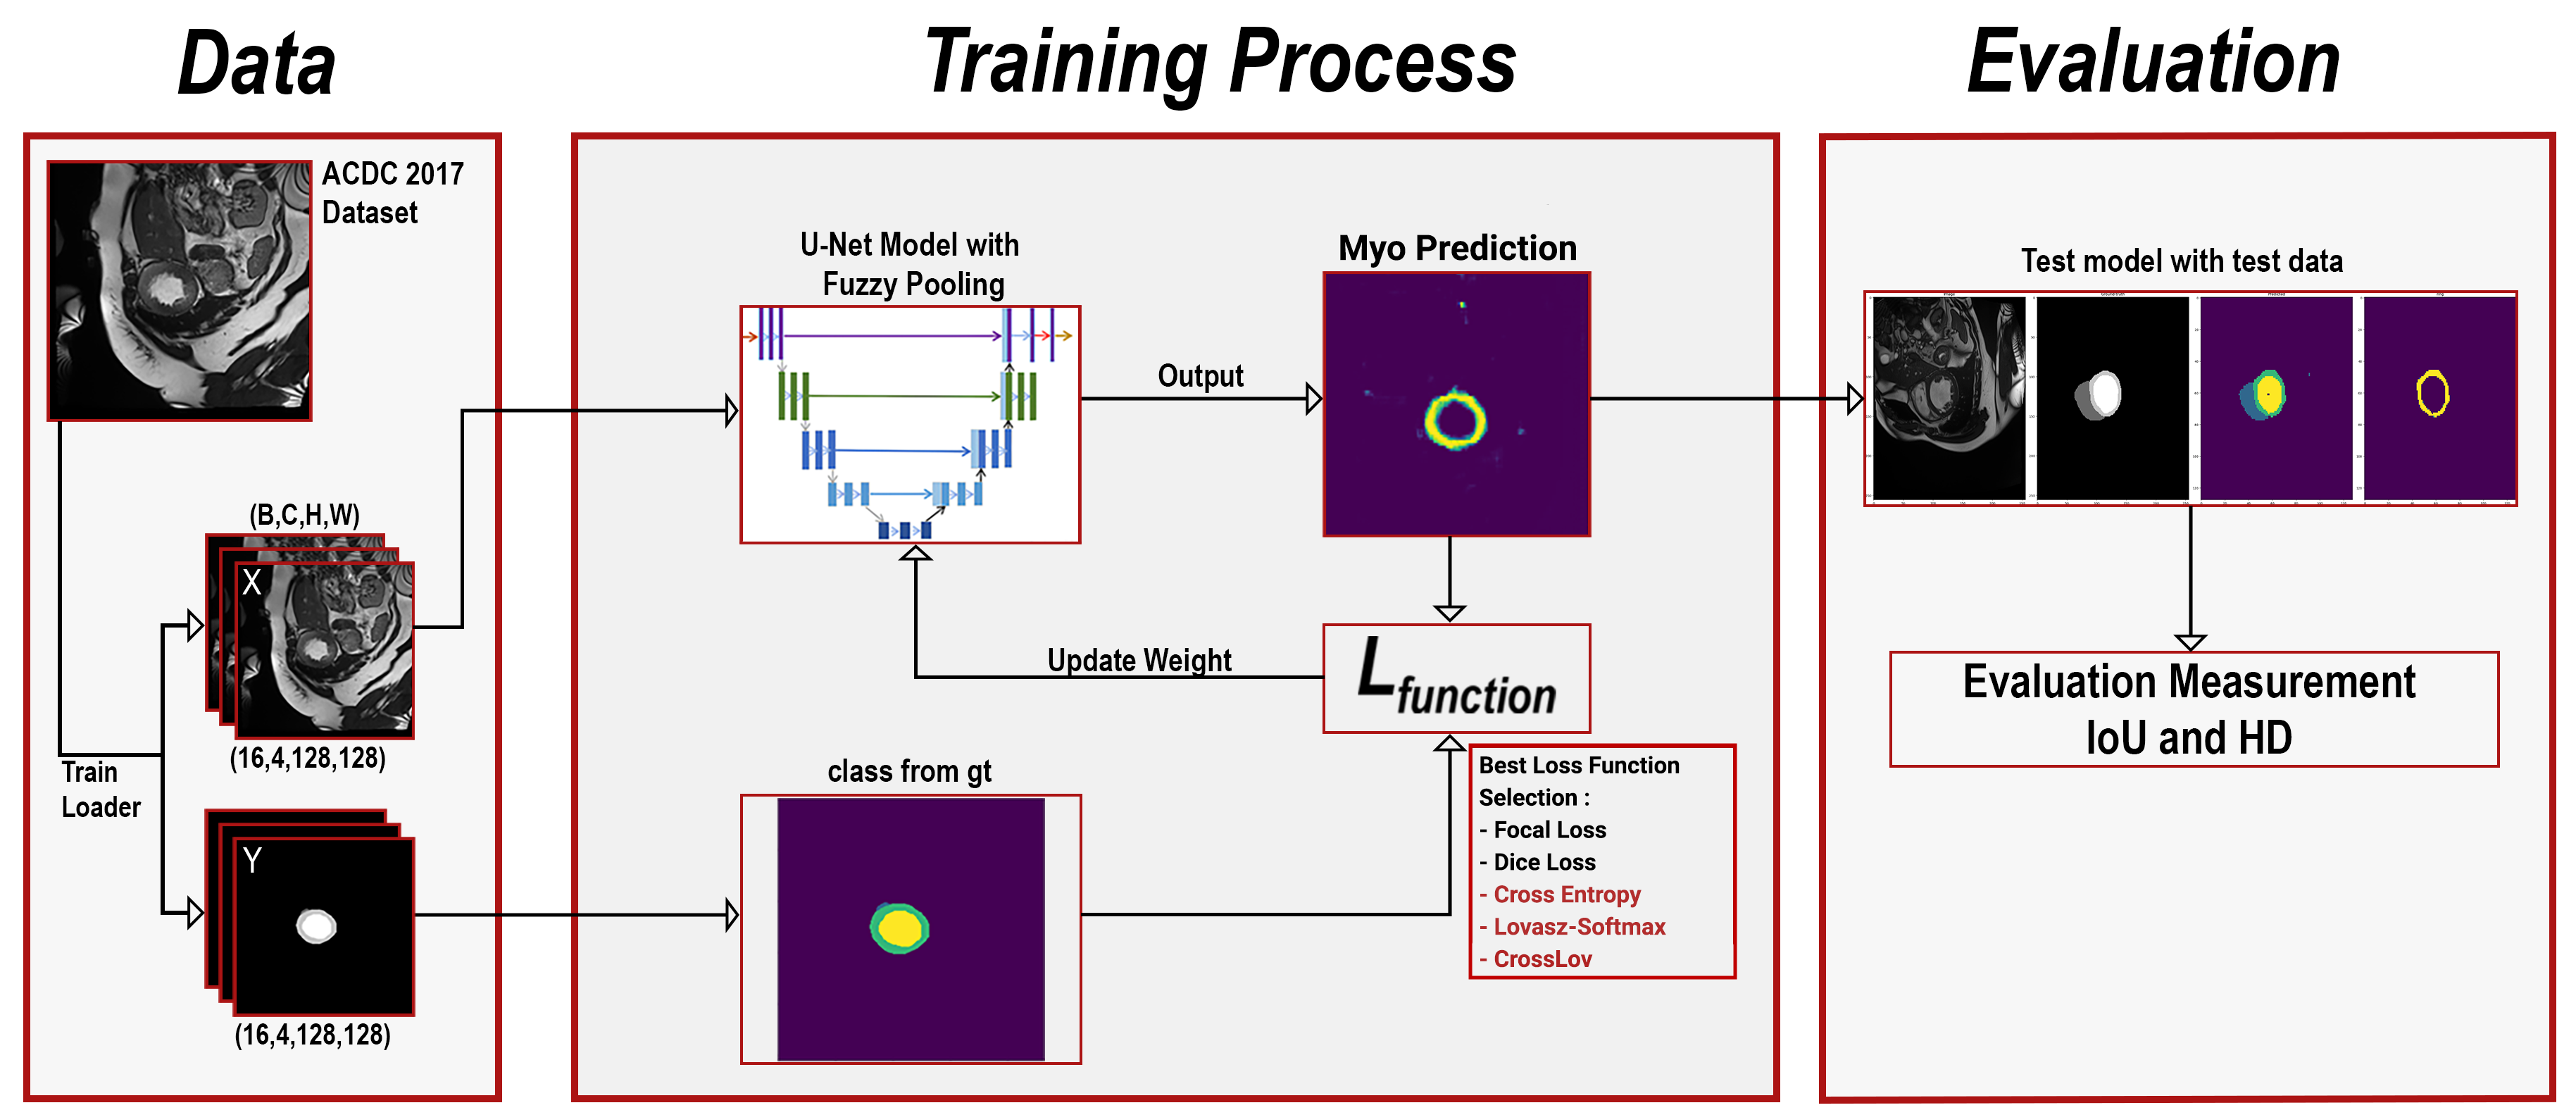
\includegraphics[width=0.86\textwidth]{bab5/ch5-framework.png}
	\caption{Overall framework for myocardium segmentation using the enhanced U-Net with fuzzy pooling and the investigated loss functions \citep{Riandini2025Array}}
	\label{fig:ch5-framework}
\end{figure}

\subsection{Fixed Enhanced U-Net with Fuzzy Pooling}
\label{subsec:ch5-fixedUnet}

The segmentation network employed throughout this chapter is identical to the enhanced U-Net with fuzzy pooling established and experimentally validated in Chapter IV. Accordingly, no architectural modifications are introduced in the present study. Instead, the previously developed segmentation network is retained as a fixed backbone to ensure that the investigated loss function remains the only independent variable affecting myocardium segmentation performance. By maintaining an identical network architecture throughout all experiments, the influence of architectural design is eliminated, enabling a fair and controlled comparison of different optimization objectives. 

The adopted network preserves the encoder-decoder architecture of the conventional U-Net while incorporating fuzzy pooling within the encoder during the down-sampling process, as illustrated in Figure~\ref{fig:ch5-architecture}. Unlike conventional max-pooling, fuzzy pooling performs feature aggregation based on fuzzy membership values, allowing representative features to be preserved while reducing the loss of spatial information during feature extraction. Combined with skip connections between the encoder and decoder, this strategy facilitates the reconstruction of anatomically consistent myocardium segmentation masks while preserving fine structural details. The effectiveness of this architecture for cardiac MR image segmentation has been demonstrated in Chapter IV and therefore serves as the fixed segmentation backbone throughout the present investigation. 

Since the primary objective of this chapter is to investigate the influence of different loss functions rather than to develop a new segmentation architecture, all architectural components are maintained without modification throughout the study. These components include the enhanced U-Net architecture, fuzzy pooling mechanism, image preprocessing procedure, optimizer, hyperparameter configuration, and dataset partition. Consequently, any observed differences in segmentation performance can be attributed exclusively to the learning behaviour of the investigated loss functions rather than to variations in network architecture or experimental settings \citep{Riandini2025Array}. 

The fuzzy pooling mechanism incorporated into the enhanced U-Net has been comprehensively described and experimentally validated in Chapter IV. Therefore, its mathematical formulation and operational procedure are not repeated in this chapter. Instead, the present investigation concentrates on how different optimization objectives influence the learning behaviour of the same segmentation network and subsequently affect myocardium segmentation performance under identical experimental conditions. 

\begin{figure}[htbp]
	\centering
	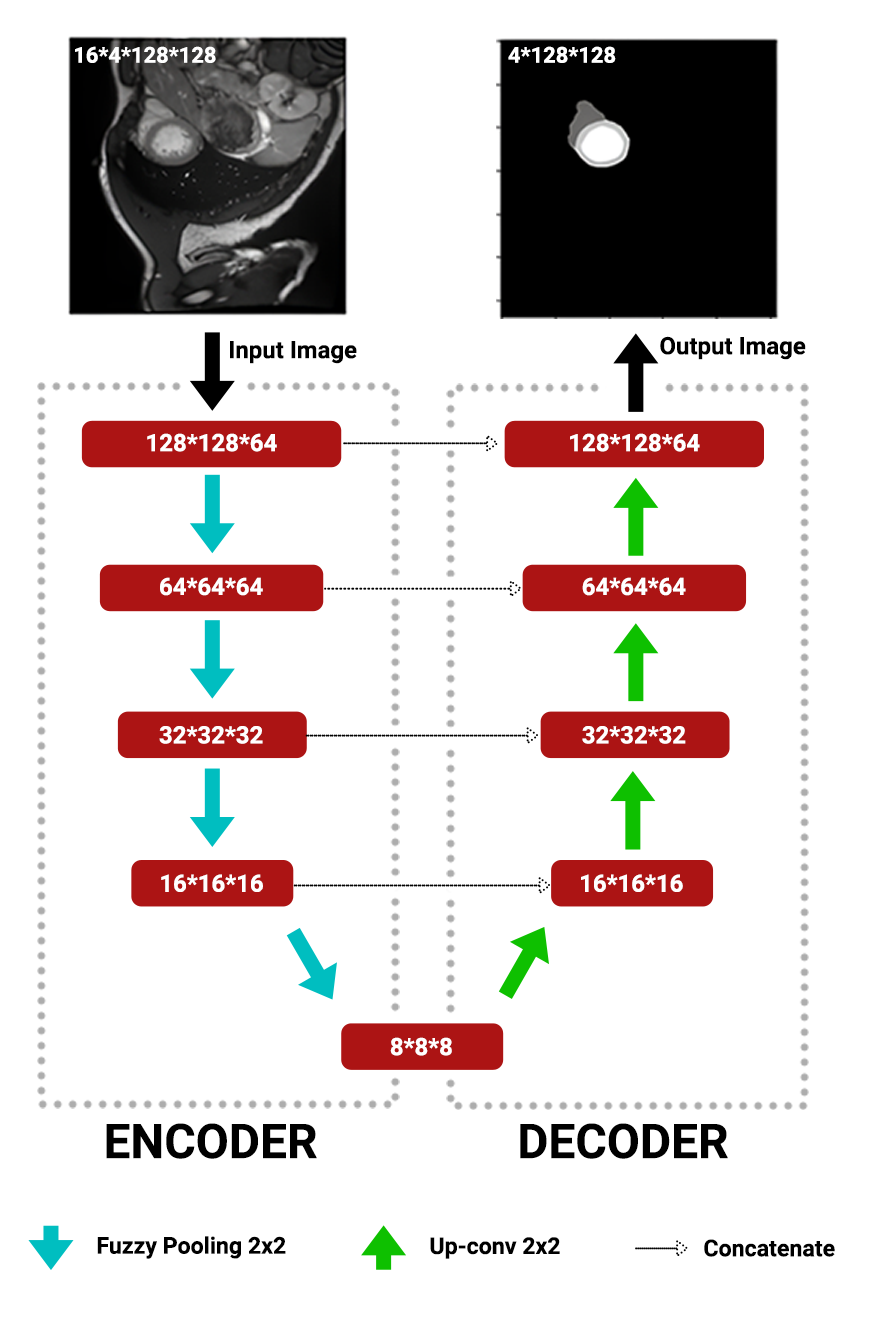
\includegraphics[width=0.86\textwidth]{bab5/ch5-architecture.png}
	\caption{Enhanced U-Net architecture applying fuzzy pooling for myocardium segmentation \citep{Riandini2025Array}}
	\label{fig:ch5-architecture}
\end{figure}

\subsection{Loss Function Investigation Strategy }
\label{subsec:ch5-LossInvestigation}

The primary objective of this chapter is to systematically investigate how different optimization objectives influence myocardium segmentation performance under an identical segmentation framework. To achieve this objective, five representative loss functions were selected based on their complementary learning characteristics, encompassing pixel-wise classification, region-overlap optimization, and hybrid learning strategies. By investigating loss functions with different optimization principles, this study aims to provide a comprehensive understanding of how the learning objective affects myocardium segmentation performance while maintaining identical network architecture and experimental settings \citep{Jadon2020,Ma2021}. 

Accordingly, five loss functions were investigated, comprising four established loss functions, namely Cross-Entropy, Dice Loss, Focal Loss, and Lovász-Softmax, together with the proposed CrossLov loss, which combines Cross-Entropy and Lovász-Softmax within a unified optimization objective. Cross-Entropy represents the conventional pixel-wise learning strategy, Dice Loss directly optimizes region overlap, Focal Loss emphasizes difficult-to-classify pixels under class imbalance, whereas Lovász-Softmax provides direct optimization of the Intersection over Union (IoU). The proposed CrossLov loss integrates pixel-wise classification with region-based optimization to exploit the complementary advantages of both learning paradigms \citep{Lin2017,Berman2018,Ma2021,Riandini2025Array}.

Based on their underlying optimization principles, the investigated loss functions can be grouped into three categories, as summarized in Table~\ref{tab:ch5-loss-classification}.

\begin{table}[htbp]
	\centering
	\caption{Classification of investigated loss functions}
	\label{tab:ch5-loss-classification}
	
	\small
	\renewcommand{\arraystretch}{1.3}
	\begin{tabular}{l l l}
		\toprule
		\textbf{Category} & \textbf{Loss Function} & \textbf{Learning Characteristic} \\
		\midrule
		Pixel-wise & Cross-Entropy & Pixel classification \\
		Pixel-wise & Focal Loss & Hard-sample emphasis \\
		Region-based & Dice Loss & Region overlap \\
		Region-based & Lov\'asz-Softmax & IoU-oriented learning \\
		Hybrid & CrossLov & Pixel-wise and region-based learning \\
		\bottomrule
		\multicolumn{3}{@{}l}{\vspace{4pt}\footnotesize \textit{Source:} Adapted from \citet{Riandini2025Array}.}
	\end{tabular}
\end{table}

As presented in Table~\ref{tab:ch5-loss-classification}, the investigated loss functions represent complementary optimization strategies. Pixel-wise loss functions focus primarily on individual pixel classification, region-based loss functions directly optimize segmentation overlap, whereas the proposed hybrid loss combines both optimization characteristics within a unified learning objective. This categorization facilitates a systematic comparison of their respective learning behaviours under identical experimental conditions while providing a conceptual basis for interpreting the quantitative and qualitative results presented in the subsequent sections. 

To ensure a fair comparative investigation, all experiments were conducted using an identical segmentation framework, including the enhanced U-Net architecture with fuzzy pooling, dataset partition, image preprocessing procedure, optimizer, hyperparameter configuration, and evaluation protocol. Consequently, the investigated loss function remained the only independent experimental variable throughout the study. The comparative analysis subsequently evaluates each loss function using training behaviour, Dice Similarity Coefficient (DSC), Intersection over Union (IoU), Hausdorff Distance (HD), and qualitative visual assessment. Collectively, these complementary evaluation criteria provide comprehensive evidence regarding the effectiveness of each investigated optimization objective for myocardium segmentation under a fixed segmentation framework \citep{Taha2015,Riandini2025Array}.

\subsection{Training Strategy }
\label{subsec:ch5-Training-Strategy}

To ensure a fair and reproducible comparative investigation, all investigated loss functions were trained under an identical training strategy. Since the objective of this chapter is to evaluate the influence of different optimization objectives on myocardium segmentation performance, every component of the segmentation framework established in Chapter IV was maintained without modification throughout all experiments. Consequently, the enhanced U-Net architecture with fuzzy pooling, dataset partition, image preprocessing procedure, optimizer, hyperparameter configuration, and evaluation protocol remained identical for every experiment. Under these controlled conditions, the investigated loss function constituted the only independent experimental variable, enabling differences in segmentation performance to be directly attributed to the learning characteristics of each optimization objective. 

The standardized training strategy adopted throughout this comparative investigation is summarized in Table~\ref{tab:ch5-training-strategy}. Each investigated loss function was independently incorporated into the training process while preserving an identical segmentation framework and experimental configuration. Maintaining consistent training conditions minimizes potential experimental bias and ensures that the observed performance differences originate exclusively from the investigated loss functions rather than from variations in network architecture or implementation settings.

\begin{table}[htbp]
	\centering
	\caption{Standardized training strategy adopted in this study}
	\label{tab:ch5-training-strategy}
	
	\small
	\renewcommand{\arraystretch}{1.3}
	\begin{tabularx}{\textwidth}{
			>{\raggedright\arraybackslash}p{0.28\textwidth}
			>{\raggedright\arraybackslash}X
		}
		\toprule
		\textbf{Training Stage} & \textbf{Purpose} \\
		\midrule
		Network initialization & Initialize the enhanced U-Net with fuzzy pooling using identical architecture and hyperparameter settings. \\ \addlinespace
		Model optimization & Train the network using one investigated loss function while maintaining identical dataset, preprocessing procedure, optimizer, learning rate, batch size, and training epochs. \\ \addlinespace
		Training monitoring & Monitor training loss, Dice Score, computational time, and the best-performing epoch throughout the training process. \\ \addlinespace
		Performance evaluation & Evaluate segmentation performance using the Dice Similarity Coefficient (DSC), Intersection over Union (IoU), Hausdorff Distance (HD), and qualitative visual assessment. \\
		\bottomrule
		\multicolumn{2}{@{}l}{\vspace{4pt}\footnotesize \textit{Source:} Adapted from \citet{Riandini2025Array}.}
	\end{tabularx}
\end{table}

Following the training process, the resulting segmentation models were evaluated using an identical assessment protocol to ensure objective comparison among the investigated loss functions. Quantitative performance was assessed using the Dice Similarity Coefficient (DSC), Intersection over Union (IoU), and Hausdorff Distance (HD), whereas qualitative evaluation was conducted through visual comparison between the predicted myocardium segmentation masks and the corresponding ground-truth annotations. In addition, the convergence behaviour of each investigated loss function was analysed by examining training loss, Dice Score, computational time, and the best-performing epoch achieved during optimization. These complementary evaluations provide a comprehensive assessment of optimization behaviour, segmentation accuracy, boundary localization, and anatomical consistency under identical experimental conditions \citep{Taha2015,Riandini2025Array}. 

By adopting a standardized training strategy throughout all comparative experiments, this study establishes a controlled experimental environment in which the influence of the investigated loss functions can be evaluated objectively and reproducibly. The training behaviour and segmentation performance obtained from this protocol are subsequently analysed in the following sections to determine the most suitable optimization objective for accurate and reliable myocardium segmentation using the enhanced U-Net framework with fuzzy pooling. 

\section{Materials and Experimental Setup}
\label{sec:ch5-Experiment-Setup}

This section describes the materials and experimental setup adopted to investigate the influence of different loss functions on myocardium segmentation performance. To ensure a fair and reproducible comparative investigation, all experiments were conducted using the same dataset, segmentation architecture, preprocessing procedure, training configuration, and evaluation protocol established in Chapter IV. Consequently, the investigated loss function remained the only independent experimental variable throughout the study, enabling differences in segmentation performance to be attributed solely to the learning characteristics of each optimization objective. The standardized experimental setup presented in this section provides the basis for interpreting the comparative results reported in the subsequent sections. 

\subsection{Dataset}
\label{subsec:ch5-Dataset}

The experimental evaluation was conducted using the Automated Cardiac Diagnosis Challenge (ACDC) 2017 dataset, which contains manually annotated cine cardiac magnetic resonance (CMR) images of the left ventricle (LV), right ventricle (RV), and myocardium (MYO). Consistent with the experimental protocol established in Chapter IV, the present study exclusively utilizes the myocardium annotations to investigate the influence of different optimization objectives on myocardium ring segmentation. By restricting the investigation to a single anatomical structure while maintaining an identical segmentation framework, the effect of the investigated loss functions can be evaluated under controlled experimental conditions. 

To maintain experimental consistency, the same dataset partition adopted in Chapter IV was retained throughout the investigation. The distribution of the training and testing images is summarized in Table~\ref{tab:ch5-dataset-distribution}.

\begin{table}[htbp]
	\centering
	\caption{Dataset distribution}
	\label{tab:dataset_distribution}
	
	\small
	\setlength{\heavyrulewidth}{\lightrulewidth}
	\renewcommand{\arraystretch}{1.3}
	\begin{tabular}{lcc}
		\toprule
		\textbf{Dataset} & \textbf{Number of Images} & \textbf{Percentage} \\
		\midrule
		Training & 1,902 & 85\% \\
		Testing & 286 & 15\% \\ \midrule
		\textbf{Total} & \textbf{2,188} & \textbf{100\%} \\ \bottomrule
		\multicolumn{3}{@{}l}{\vspace{4pt}\footnotesize \textit{Source:} Adapted from \citet{Riandini2026Access}.}
	\end{tabular}
\end{table}

All preprocessing procedures, including image normalization, resizing, and annotation preparation, were performed identically for every investigated loss function. Maintaining an identical preprocessing pipeline ensures that variations in segmentation performance originate exclusively from differences in the adopted optimization objective rather than from inconsistencies in data preparation. 

\subsection{Experimental Environment}
\label{subsec:ch5-experiment-enviroment}

All comparative experiments were conducted using an identical computational environment to ensure consistency during model training and performance evaluation. The hardware and implementation settings employed throughout the investigation are summarized in Table~\ref{tab:ch5-experiment-environment}.

\begin{table}[htbp]
	\centering
	\caption{Experimental Environment}
	\label{tab:experimental_environment}
	
	\small
	\setlength{\heavyrulewidth}{\lightrulewidth}
	\renewcommand{\arraystretch}{1.3}
	
	% \resizebox DIHAPUS agar tabel tidak ditarik melar
	\begin{tabular}{ll}
		\toprule
		\textbf{Component} & \textbf{Specification} \\ \midrule
		GPU                 & Tesla T4 \\
		GPU Memory          & 32 GB \\
		Training Epochs     & 100 \\
		Input Tensor Format & $16 \times 4 \times 128 \times 128$ \\ \bottomrule
	\end{tabular}
\end{table}

The computational environment presented in Table~\ref{tab:ch5-experiment-environment} was maintained without modification for all comparative experiments. Consequently, the computational performance and segmentation accuracy obtained by each investigated loss function were evaluated under identical hardware conditions, thereby ensuring a fair comparison of the resulting optimization behaviour. 

\subsection{Training Configuration}
\label{subsec:ch5-training-config}

To ensure a fair comparative investigation, every investigated loss function was trained using an identical network configuration. Apart from the optimization objective, all components of the segmentation framework, including the enhanced U-Net architecture, fuzzy pooling mechanism, preprocessing procedure, optimizer, dataset partition, and hyperparameter configuration, were maintained without modification throughout the study. The adopted training configuration is summarized in Table~\ref{tab:ch5-training-config}.

\begin{table}[htbp]
	\centering
	\caption{Training configuration adopted in this study}
	\label{tab:ch5-training-config}
	
	\small
	\setlength{\heavyrulewidth}{\lightrulewidth}
	\renewcommand{\arraystretch}{1.3}
	\begin{tabularx}{\textwidth}{
			>{\raggedright\arraybackslash}p{0.32\textwidth}
			>{\raggedright\arraybackslash}X
		}
		\toprule
		\textbf{Parameter} & \textbf{Configuration} \\
		\midrule
		Segmentation Network & Enhanced U-Net \\
		Pooling Method & Fuzzy Pooling \\
		Target Structure & Myocardium (MYO) \\
		Input Image Size & 128 $\times$ 128 pixels \\
		Number of Classes & 4 \\
		Batch Size & 16 \\
		Investigated Loss Functions & Cross-Entropy, Dice Loss, Focal Loss, Lov\'asz-Softmax, CrossLov \\
		Training Epochs & 100 \\
		\bottomrule
		\multicolumn{2}{@{}l}{\vspace{4pt}\footnotesize \textit{Source:} Adapted from \citet{Riandini2025Array}.}
	\end{tabularx}
\end{table}

The standardized configuration summarized in Table~\ref{tab:ch5-training-config} ensures that the investigated loss function remains the only experimental factor differing among all training sessions. Therefore, any observed differences in segmentation performance can be interpreted as the consequence of the adopted optimization objective rather than differences in network architecture or training settings. 

\subsection{Evaluation Metrics}
\label{subsec:ch5-eval-metric}

The effectiveness of each investigated loss function was evaluated using quantitative metrics that are widely employed in medical image segmentation studies. To provide complementary assessments of segmentation performance, overlap-based and boundary-based metrics were jointly adopted. The evaluation metrics used throughout this study are summarized in Table~\ref{tab:ch5-eval-metric}.

\begin{table}[htbp]
	\centering
	\caption{Evaluation metrics used in this study}
	\label{tab:ch5-eval-metric}
	
	\small
	\setlength{\heavyrulewidth}{\lightrulewidth}
	\renewcommand{\arraystretch}{1.3}
	\begin{tabularx}{\textwidth}{
			>{\raggedright\arraybackslash}p{0.32\textwidth}
			>{\raggedright\arraybackslash}X
		}
		\toprule
		\textbf{Metric} & \textbf{Purpose} \\
		\midrule
		Dice Similarity Coefficient (DSC) & Measures the overlap between the predicted segmentation and the ground-truth annotation. \\ \addlinespace
		Intersection over Union (IoU) & Evaluates regional agreement between the predicted myocardium segmentation and the reference annotation. \\ \addlinespace
		Hausdorff Distance (HD) & Measures the maximum boundary distance between the predicted segmentation and the reference annotation. \\
		\bottomrule
		\multicolumn{2}{@{}l}{\vspace{4pt}\footnotesize \textit{Source:} Adapted from \citet{Taha2015}.}
	\end{tabularx}
\end{table}

In addition to quantitative evaluation, qualitative visual assessment was performed by comparing the predicted myocardium segmentation masks with the corresponding ground-truth annotations. The combination of quantitative measurements and visual inspection provides a more comprehensive understanding of segmentation performance, particularly for assessing boundary continuity and anatomical consistency. The comparative results obtained using these evaluation criteria are presented and discussed in the following section. 

\section{Experimental Results and Discussion}
\label{sec:ch5-experiment-result-discuss}

This section presents a comparative analysis of the investigated loss functions using identical experimental conditions. The discussion is organized according to the experimental evidence obtained from the training process, quantitative evaluation, and qualitative visual assessment. By maintaining the same segmentation framework throughout the investigation, the observed performance differences can be attributed solely to the investigated loss functions.

\subsection{Training Behaviour Analysis}
\label{subsec:ch5-training-analysis}

Before comparing the final segmentation performance achieved by the investigated loss functions, it is essential to first analyse their behaviour during the network training process. Although all comparative experiments were conducted using the same enhanced U-Net architecture, fuzzy pooling strategy, dataset partition, preprocessing procedure, optimizer, hyperparameter configuration, and training protocol, the optimization behaviour varies according to the selected loss function. Consequently, analysing the training process provides valuable insight into convergence stability, learning efficiency, computational cost, and segmentation capability before evaluating the final quantitative and qualitative segmentation results.
The training behaviour of the five investigated loss functions is presented in Figure~\ref{fig:ch5-training-performance}, which summarizes the evolution of the training loss, testing loss, Dice score, computational time, and the best-performing training epoch obtained under identical experimental conditions.

\begin{figure}[htbp]
	\centering
	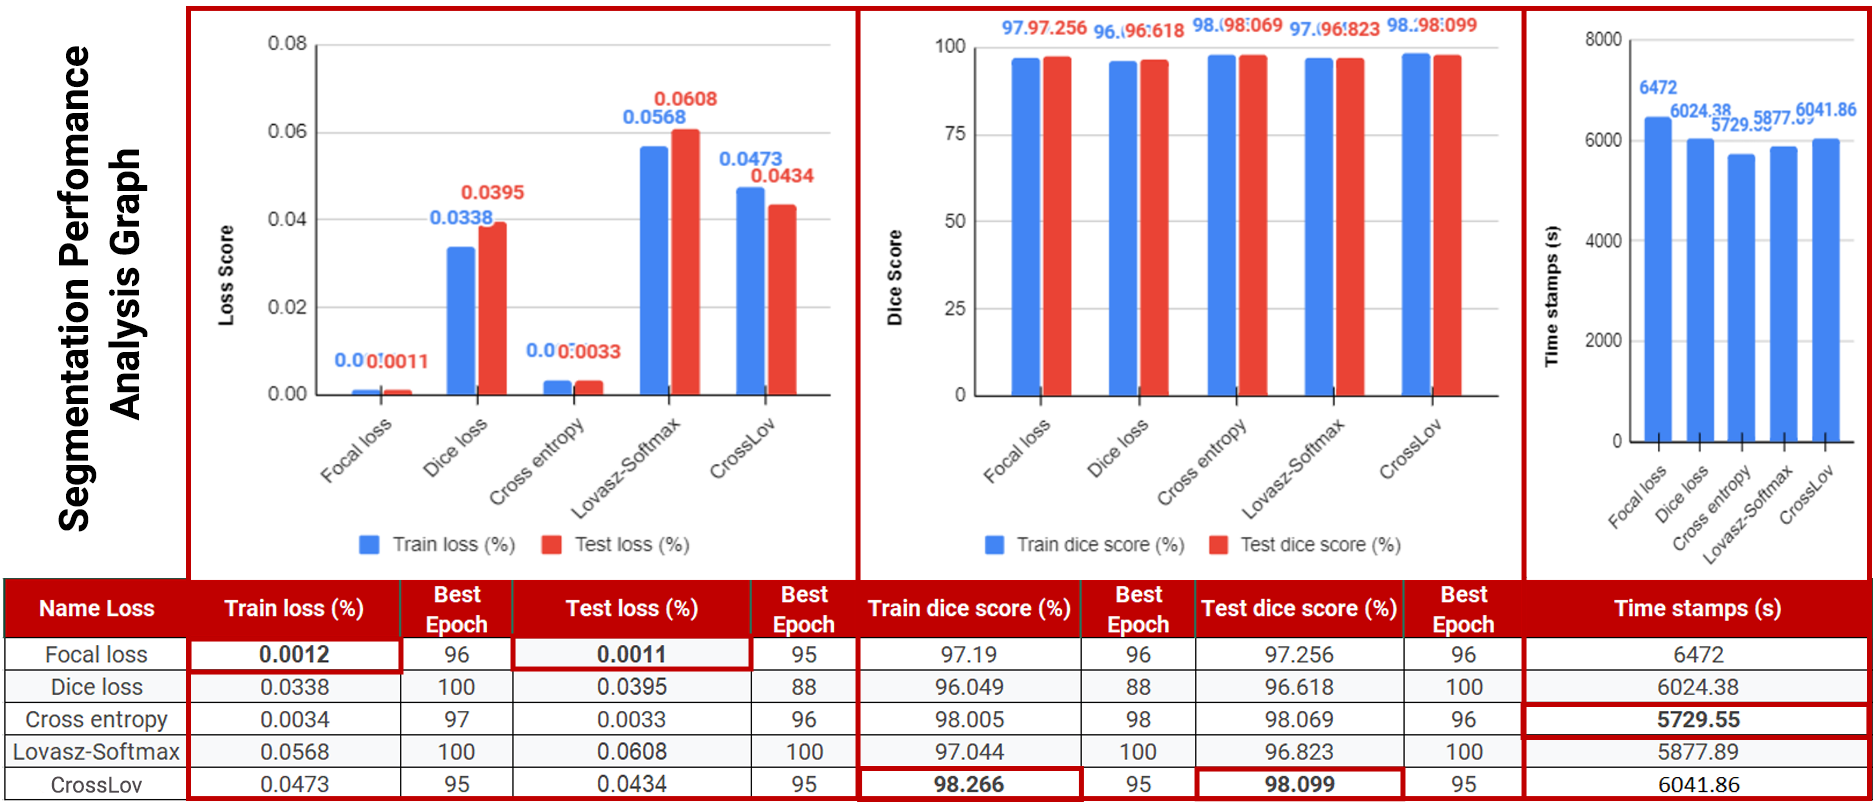
\includegraphics[width=\textwidth]{bab5/ch5-training-performance.png}
	\caption{Training performance of the investigated loss functions showing the training loss, testing loss, Dice score, computational time, and best-performing epoch obtained for each evaluated loss function \protect\citep{Riandini2025Array}}
	\label{fig:ch5-training-performance}
\end{figure}

As illustrated in Figure~\ref{fig:ch5-training-performance}, the investigated loss functions demonstrate noticeably different optimization behaviours despite being trained using an identical segmentation framework. The training and testing loss curves indicate that Focal Loss consistently achieved the smallest objective function values throughout the optimization process, suggesting that it was highly effective in minimizing prediction error during learning. However, the reduction of the optimization objective did not necessarily correspond to the highest segmentation accuracy, indicating that convergence of the loss function alone is insufficient to evaluate segmentation performance comprehensively.

A different trend is observed from the Dice score analysis. While Focal Loss produced the lowest optimization loss, CrossLov consistently achieved the highest Dice score for both the training and testing datasets. This observation suggests that combining Cross-Entropy and Lovász-Softmax enables the optimization process to simultaneously preserve pixel-wise classification accuracy and region-level overlap. Consequently, CrossLov generated more accurate myocardium segmentation even though its optimization loss was not the smallest among the investigated methods.

Figure~\ref{fig:ch5-training-performance} also reveals differences in computational efficiency. Among the investigated loss functions, Cross-Entropy required the shortest training time to complete the full optimization process, whereas Focal Loss required the longest computational time under the same hardware configuration. Although the computational difference is relatively modest, this observation indicates that optimization objectives emphasizing difficult samples may require additional computational resources during training.

To facilitate interpretation of the training behaviour illustrated in Figure~\ref{fig:ch5-training-performance}, the principal observations are summarized in  Table~\ref{tab:ch5-summary-training-behaviour}.

\begin{table}[htbp]
	\centering
	\caption{Summary of Training Behaviour based on Figure~\ref{fig:ch5-training-performance}}
	\label{tab:ch5-summary-training-behaviour}
	
	\small
	\setlength{\heavyrulewidth}{\lightrulewidth}
	\renewcommand{\arraystretch}{1.3}
	
	% \resizebox DIHAPUS agar font kembali ke ukuran normal/proporsional
	\begin{tabular}{ll}
		\toprule
		\textbf{Observation} & \textbf{Result} \\ \midrule
		Lowest Training Loss       & Focal Loss (0.0012, Epoch 96) \\
		Lowest Testing Loss        & Focal Loss (0.0011, Epoch 95) \\
		Highest Training Dice Score & CrossLov (98.266\%, Epoch 95) \\
		Highest Testing Dice Score  & CrossLov (98.099\%, Epoch 95) \\
		Shortest Training Time     & Cross-Entropy (5729.55 s) \\
		Longest Training Time      & Focal Loss (6472 s) \\ \bottomrule
	\end{tabular}
\end{table}

The observations summarized in Table~\ref{tab:ch5-summary-training-behaviour} confirm that each investigated loss function exhibits distinct optimization characteristics despite sharing an identical segmentation framework. Focal Loss demonstrated superior convergence behaviour by minimizing the optimization objective more effectively than the remaining methods, whereas Cross-Entropy provided the highest computational efficiency by requiring the shortest training time. In contrast, CrossLov consistently achieved the highest Dice scores on both the training and testing datasets, indicating that balanced optimization of pixel-wise classification and region-level overlap contributes more effectively to segmentation accuracy than minimizing the loss function alone.

These findings demonstrate that convergence behaviour, computational efficiency, and segmentation accuracy represent complementary aspects of optimization performance rather than interchangeable evaluation criteria. A loss function producing the smallest optimization error does not necessarily generate the highest-quality segmentation results, while rapid convergence does not automatically indicate superior anatomical representation. Therefore, comprehensive evaluation using segmentation-oriented performance metrics is required to determine the most appropriate optimization objective for myocardium segmentation.

The influence of each investigated loss function on segmentation accuracy is further analysed quantitatively in the following section using the \textbf{Dice Similarity Coefficient (DSC)}, Intersection \textbf{over Union (IoU)}, and \textbf{Hausdorff Distance (HD)} to provide a comprehensive comparison of overlap accuracy and boundary consistency.

\subsection{Quantitative Comparison of Loss Functions}
\label{subsec:ch5-quantitative-compare-loss}

The quantitative performance of the investigated loss functions was evaluated using the Dice Similarity Coefficient (DSC), Intersection over Union (IoU), and Hausdorff Distance (HD). These complementary metrics provide comprehensive assessment of segmentation performance by simultaneously evaluating regional overlap and boundary agreement between the predicted myocardium segmentation and the corresponding ground-truth annotation. The complete quantitative results obtained under identical experimental conditions are presented in Table~\ref{tab:ch5-quantitative-compare-loss}.

\begin{sidewaystable}[htbp]
	\centering
	\caption{Evaluation results of state-of-the-art models and proposed CrossLov using IoU, HD, and Dice Score}
	\label{tab:ch5-quantitative-compare-loss}
	
	% 1. Ubah font menjadi lebih kecil satu tingkat agar muat di margin
	\footnotesize 
	% 2. Rapatkan jarak antar kolom secara signifikan
	\setlength{\tabcolsep}{3pt} 
	\setlength{\heavyrulewidth}{\lightrulewidth}
	% 3. Kurangi sedikit padding vertikal
	\renewcommand{\arraystretch}{1.15} 
	
	\begin{tabular}{llccccc}
		\toprule
		\textbf{Evaluation metric} & \textbf{Class} & \multicolumn{5}{c}{\textbf{Name loss}} \\ \cmidrule(lr){3-7}
		& & \specialcell{\textbf{Focal Loss} \\ \citep{Lin2017}} & \specialcell{\textbf{Dice Loss} \\ \citep{Wyburd2021,Ma2021}} & \specialcell{\textbf{Cross entropy} \\ \citep{Yeung2022}} & \specialcell{\textbf{Lovasz-Softmax} \\ \citep{Berman2018}} & \textbf{CrossLov} \\
		\midrule
		\multirow{2}{*}{Average IoU (\%)} & MYO + LV + RV & 91.862 & 87.647 & 81.103 & 88.763 & \textbf{93.691} \\
		& MYO & 51.965 & 89.4 & 51.959 & \textbf{90.68} & 60.262 \\ \addlinespace
		\multirow{2}{*}{Highest IoU (\%)} & MYO + LV + RV & \textbf{100} & 95.909 & 94.54 & 97.757 & \textbf{100} \\
		& MYO & \textbf{100} & \textbf{100} & \textbf{100} & \textbf{100} & \textbf{100} \\ \addlinespace
		\multirow{2}{*}{Lowest IoU (\%)} & MYO + LV + RV & 49.972 & 33.274 & 33.3 & 34.955 & \textbf{49.987} \\
		& MYO & 48.3 & \textbf{67.152} & 49.148 & 49.88 & 49.633 \\ \addlinespace
		\multirow{2}{*}{Average HD} & MYO + LV + RV & 2.935 & 3.27 & 4.598 & 3.251 & \textbf{2.816} \\
		& MYO & 1.338 & 1.648 & 1.689 & 1.527 & \textbf{1.309} \\ \addlinespace
		\multirow{2}{*}{Highest HD} & MYO + LV + RV & 4.242 & 6 & 4 & 8.062 & 6.928 \\
		& MYO & 1.746 & 2.922 & \textbf{1.734} & 2.862 & 2.221 \\ \addlinespace
		\multirow{2}{*}{Lowest HD} & MYO + LV + RV & \textbf{1} & \textbf{1} & \textbf{0} & 0.43 & 0.0004 \\
		& MYO & 0.012 & \textbf{3.60E-06} & 7.63E-03 & -- & 97.256 \\ \addlinespace
		Dice score & & 96.823 & 96.618 & 98.069 & 96.823 & \textbf{98.099} \\
		\bottomrule
		\multicolumn{7}{@{}l}{\vspace{4pt}\textit{Source:} Adapted from \citet{Riandini2025Array}.}
	\end{tabular}
\end{sidewaystable}

The quantitative results presented in Table~\ref{tab:ch5-quantitative-compare-loss} demonstrate that the investigated loss functions exhibit different optimization characteristics depending on the evaluation metric considered. Although all experiments employed an identical segmentation framework, variations in the optimization objective resulted in measurable differences in overlap accuracy and boundary consistency. To facilitate interpretation of these findings, the principal quantitative observations are summarized in Table~\ref{tab:ch5-summary-quantitative-performance}.

\begin{table}[htbp]
	\centering
	\caption{Summary of Quantitative Performance based on Table~\ref{tab:ch5-quantitative-compare-loss}}
	\label{tab:ch5-summary-quantitative-performance}
	
	\small
	% Menyamakan ketebalan garis booktabs agar seragam tipis
	\setlength{\heavyrulewidth}{\lightrulewidth}
	% Memberikan padding vertikal yang lega (tidak menjepit judul kolom)
	\renewcommand{\arraystretch}{1.3}
	
	\resizebox{\linewidth}{!}{%
		\begin{tabular}{lll}
			\toprule
			\textbf{Evaluation Criterion} & \textbf{Best Result} & \textbf{Loss Function} \\ \midrule
			Average IoU (MYO + LV + RV)   & 93.691\%             & CrossLov \\
			Average IoU (MYO)             & 90.680\%             & Lov\'asz-Softmax \\
			Lowest Average HD (MYO + LV + RV) & 2.816             & CrossLov \\
			Lowest Average HD (MYO)       & 1.309                & CrossLov \\
			Highest Dice Score            & 98.099\%             & CrossLov \\ \bottomrule
		\end{tabular}%
	}
\end{table}

The summary presented in Table~\ref{tab:ch5-summary-quantitative-performance} indicates that no single loss function consistently achieved the best result for every evaluation criterion. Instead, each investigated optimization objective emphasized different aspects of myocardium segmentation performance. Lovász-Softmax achieved the highest Average IoU for myocardium segmentation, indicating its effectiveness in maximizing regional overlap between the predicted myocardium and the reference annotation. This observation is consistent with the optimization objective of \textbf{Lovász-Softmax}, which directly approximates the IoU metric during network training.

In contrast, \textbf{CrossLov} demonstrated the most balanced overall performance across the evaluated metrics. In addition to achieving the highest Dice Similarity Coefficient, CrossLov also produced the lowest Hausdorff Distance for both the overall cardiac structures and the myocardium. These findings indicate that the combination of Cross-Entropy and Lovász-Softmax enables the network to preserve accurate pixel-wise classification while simultaneously improving regional overlap and boundary localization. Consequently, the resulting segmentation masks exhibit both high overlap accuracy and improved anatomical consistency.

The quantitative evaluation also confirms the observations obtained from the training behaviour analysis presented in the previous subsection. Although \textbf{Focal Loss} produced the smallest optimization loss during network training and \textbf{Cross-Entropy} required the shortest computational time, neither approach consistently achieved the highest segmentation performance according to the quantitative evaluation metrics. This finding further demonstrates that convergence behaviour alone is insufficient to represent segmentation quality and should always be interpreted together with overlap-based and boundary-based evaluation metrics.
Overall, the quantitative comparison demonstrates that different loss functions optimize different characteristics of myocardium segmentation. Whereas Lovász-Softmax primarily improves regional overlap, CrossLov provides a more balanced optimization strategy by simultaneously achieving excellent overlap accuracy and superior boundary agreement. These findings suggest that combining complementary optimization objectives is more effective than relying on a single loss formulation when accurate and anatomically consistent myocardium segmentation is required.

The quantitative findings presented in this section provide objective evidence of the influence of the investigated loss functions on segmentation performance. Nevertheless, numerical evaluation alone cannot fully illustrate the visual quality of the generated myocardium contours. Therefore, a qualitative visual assessment is presented in the following section to examine the anatomical appearance of the predicted segmentation masks and to verify whether the quantitative improvements are consistently reflected in the resulting segmentation outcomes.

\subsection{Visual Segmentation Analysis}
\label{subsec:ch5-visual-seg-analysis}

Although quantitative evaluation provides objective measurements of segmentation performance, numerical metrics alone cannot fully illustrate the anatomical quality of the generated myocardium segmentation. Therefore, qualitative visual assessment was performed by comparing the predicted myocardium segmentation masks with their corresponding ground-truth annotations. This complementary analysis enables visual verification of whether the improvements observed in the quantitative evaluation are consistently reflected in the anatomical appearance of the resulting segmentation masks.

The representative qualitative comparison of the investigated loss functions is presented in Figure~\ref{fig:ch5-visual-seg-analysis}.

\begin{comment}
\begin{figure}[htbp]
	\centering
	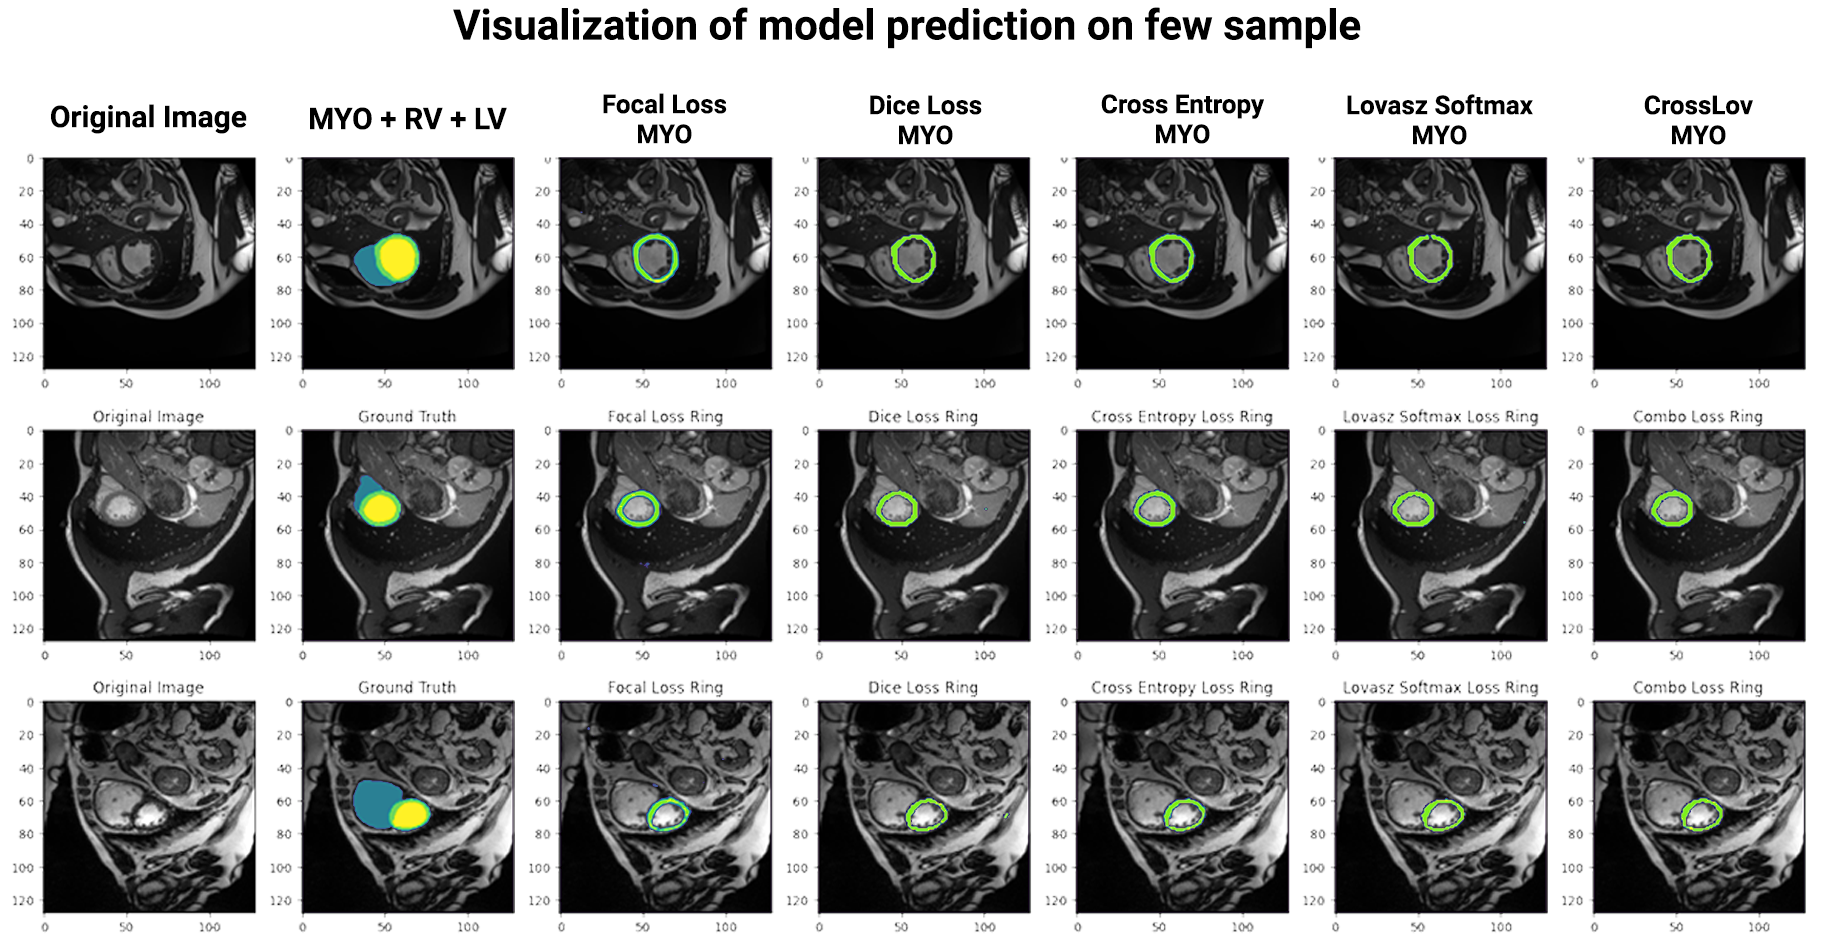
\includegraphics[width=0.86\textwidth]{bab5/ch5-visual-seg-analysis.png}
	\caption{Visual comparison of myocardium segmentation results obtained using the investigated loss functions. The predicted myocardium segmentation is shown in red, whereas the corresponding ground-truth annotation is shown in green \citep{Riandini2025Array}}
	\label{fig:ch5-visual-seg-analysis}
\end{figure}
\end{comment}

\begin{sidewaysfigure}[htbp]
	\centering
	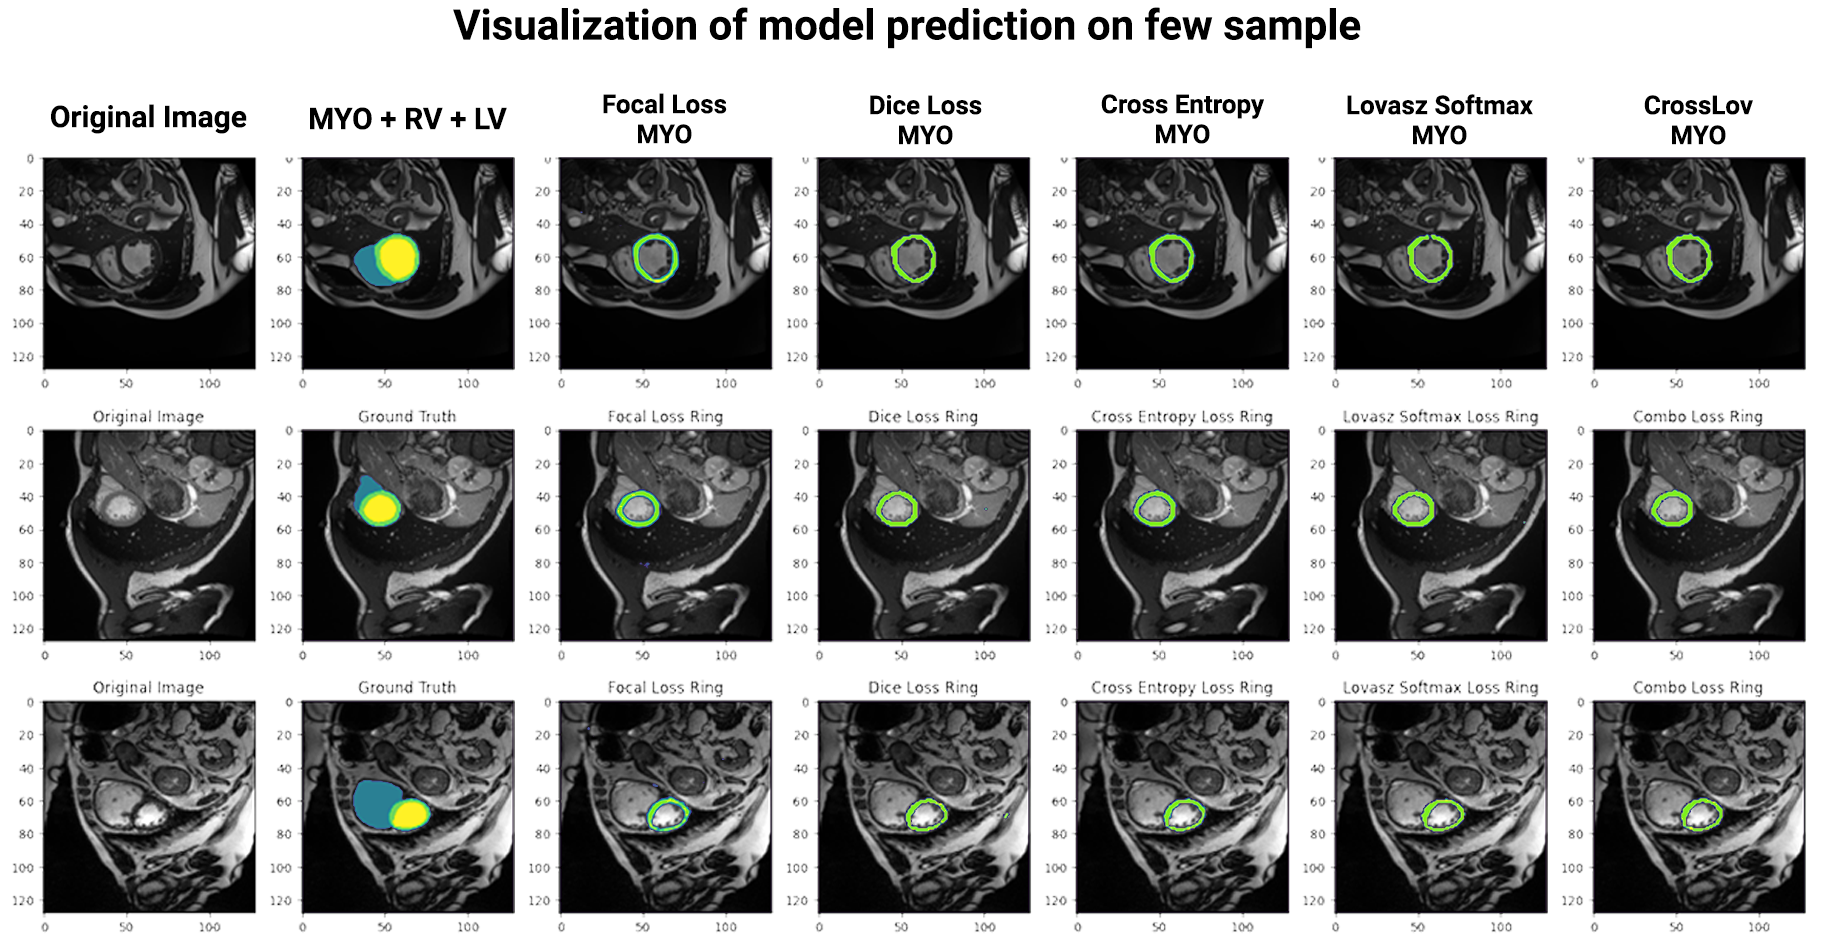
\includegraphics[width=\textwidth]{bab5/ch5-visual-seg-analysis.png}
	\caption{Visual comparison of myocardium segmentation results obtained using the investigated loss functions. The predicted myocardium segmentation is shown in red, whereas the corresponding ground-truth annotation is shown in green \protect\citep{Riandini2025Array}}
	\label{fig:ch5-visual-seg-analysis}
\end{sidewaysfigure}

As illustrated in Figure~\ref{fig:ch5-visual-seg-analysis}, all investigated loss functions successfully identified the myocardium region under identical experimental conditions. Nevertheless, noticeable differences can be observed in the continuity of the predicted myocardial contours and their agreement with the corresponding reference annotations. These visual differences demonstrate that the choice of optimization objective influences not only numerical evaluation metrics but also the anatomical appearance of the resulting segmentation masks.

The visual comparison indicates that \textbf{Cross-Entropy}, \textbf{Focal Loss}, and \textbf{Dice Loss} produced generally acceptable segmentation results but still exhibited visible discrepancies between the predicted contours and the reference annotations in several representative examples. Although these deviations are relatively small, they indicate that optimization based on a single learning objective may not consistently preserve both regional overlap and boundary accuracy.

In comparison, \textbf{Lovász-Softmax} generated segmentation masks that more closely followed the myocardial region, reflecting its superior regional overlap observed during the quantitative evaluation. This behaviour is consistent with the optimization objective of Lovász-Softmax, which directly promotes improved Intersection over Union (IoU) during network training. Consequently, the predicted myocardium contours demonstrate closer agreement with the reference annotation in terms of regional coverage.

Among the investigated approaches, \textbf{CrossLov} demonstrated the closest overall visual agreement with the corresponding ground-truth annotations. The predicted myocardial contours appear more continuous and more closely aligned with the anatomical boundaries of the reference segmentation, indicating improved consistency between overlap accuracy and boundary localization. These visual observations are consistent with the quantitative findings presented in the previous subsection, where CrossLov achieved the highest Dice Similarity Coefficient together with the lowest Hausdorff Distance among the investigated loss functions.

To facilitate interpretation of the qualitative observations presented in Figure~\ref{fig:ch5-visual-seg-analysis}, the principal visual findings are summarized in Table~\ref{tab:ch5-visual-assessment}.

\begin{table}[htbp]
	\centering
	\caption{Summary of visual assessment based on Figure 5.4}
	\label{tab:ch5-visual-assessment}
	
	\small
	\setlength{\heavyrulewidth}{\lightrulewidth}
	\renewcommand{\arraystretch}{1.3}
	\begin{tabularx}{\textwidth}{
			>{\raggedright\arraybackslash}p{0.22\textwidth}
			>{\raggedright\arraybackslash}X
			>{\raggedright\arraybackslash}X
		}
		\toprule
		\textbf{Loss Function} & \textbf{Visual Observation} & \textbf{Consistency with Quantitative Results} \\
		\midrule
		Cross-Entropy & Relatively consistent segmentation with minor discrepancies. & Consistent with moderate IoU and HD performance. \\ \addlinespace
		Focal Loss & Stable prediction but visible deviations in several samples. & Consistent with low training loss but moderate segmentation performance. \\ \addlinespace
		Dice Loss & Good regional overlap with several contour inconsistencies. & Consistent with competitive quantitative performance. \\ \addlinespace
		Lov\'asz-Softmax & Segmentation closely follows the myocardium region. & Consistent with the highest myocardium IoU. \\ \addlinespace
		CrossLov & Closest visual agreement with the reference annotation. & Consistent with the highest Dice Score and lowest HD. \\
		\bottomrule
	\end{tabularx}
\end{table}

The qualitative observations summarized in Table~\ref{tab:ch5-visual-assessment} demonstrate strong agreement with the quantitative evaluation presented in Section~\ref{subsec:ch5-quantitative-compare-loss}. The quantitative results are reflected in Dice Similarity Coefficient, Intersection over Union, and Hausdorff Distance are reflected in the visual appearance of the generated myocardium segmentation masks. In particular, the balanced quantitative performance achieved by CrossLov is accompanied by more consistent contour continuity and closer agreement with the reference annotations, whereas the strengths of Lovász-Softmax are primarily reflected in higher regional overlap.

Overall, the qualitative assessment confirms that the investigated loss functions influence not only quantitative segmentation accuracy but also the anatomical quality of the resulting myocardium segmentation. The consistency between the quantitative evaluation and the visual observations strengthens the reliability of the experimental findings and provides additional evidence that an appropriate optimization objective contributes substantially to accurate and anatomically consistent myocardium segmentation.

The findings obtained from the training behaviour analysis, quantitative evaluation, and qualitative visual assessment are integrated in the following section to provide a comprehensive discussion of the influence of the investigated loss functions on myocardium segmentation performance.

\begin{table}[htbp]
	\centering
	\caption{Summary of training behaviour}
	\label{tab:ch5-training-behaviour}
	
	\small
	\setlength{\heavyrulewidth}{\lightrulewidth}
	\renewcommand{\arraystretch}{1.3}
	\begin{tabularx}{\textwidth}{
			>{\raggedright\arraybackslash}p{0.45\textwidth}
			>{\raggedright\arraybackslash}X
		}
		\toprule
		\textbf{Observation} & \textbf{Result} \\
		\midrule
		Lowest Training Loss & Focal Loss (0.0012, Epoch 96) \\
		Lowest Testing Loss & Focal Loss (0.0011, Epoch 95) \\
		Highest Training Dice Score & CrossLov (98.266) \\
		Highest Testing Dice Score & CrossLov (98.099) \\
		Shortest Training Time & Cross-Entropy (5729.55 s) \\
		Longest Training Time & Focal Loss (6472 s) \\
		\bottomrule
	\end{tabularx}
\end{table}

\subsection{Overall Discussion}
\label{subsec:ch5-discussion}  

The experimental results presented throughout this chapter demonstrate that the selection of an appropriate loss function substantially influences myocardium segmentation performance, even when the segmentation architecture, preprocessing procedure, dataset partition, and training configuration remain unchanged. Since all comparative experiments employed an identical enhanced U-Net framework with fuzzy pooling, the observed differences in segmentation performance can be attributed exclusively to the investigated optimization objectives. These findings confirm that segmentation quality depends not only on the capability of the network architecture to extract representative image features but also on how the optimization objective guides the learning process during network training.

The training behaviour analysis presented in  Section~\ref{subsec:ch5-training-analysis} demonstrates that convergence of the optimization loss alone is insufficient to represent segmentation quality. Although \textbf{Focal Loss} consistently achieved the smallest training and testing loss values, it did not produce the highest segmentation accuracy according to the quantitative evaluation. Conversely, \textbf{CrossLov} achieved the highest Dice Similarity Coefficient despite not producing the lowest optimization loss. This observation indicates that minimizing the optimization objective does not necessarily maximize agreement between the predicted segmentation and the corresponding ground-truth annotation. Consequently, evaluating segmentation performance solely on the basis of convergence behaviour may lead to incomplete interpretation of model performance.

The quantitative evaluation further demonstrates that different optimization objectives emphasize different characteristics of myocardium segmentation. \textbf{Lovász-Softmax} achieved the highest Intersection over Union for myocardium segmentation, reflecting its capability to achieve higher regional overlap through direct optimization of an IoU-oriented objective. In contrast, \textbf{CrossLov} consistently achieved the highest Dice Similarity Coefficient together with the lowest Hausdorff Distance, indicating a more balanced capability to preserve both overlap accuracy and boundary consistency. The findings suggest that combining complementary optimization objectives provides a balanced trade-off between overlap accuracy and boundary localization.

The qualitative visual assessment further strengthens these findings. The segmentation masks generated using \textbf{CrossLov} demonstrated closer agreement with the reference annotations, exhibiting smoother myocardial contours and improved boundary continuity compared with the remaining investigated loss functions. Meanwhile, the segmentation masks produced by \textbf{Lovász-Softmax} reflected its superior regional overlap, whereas the remaining loss functions exhibited minor discrepancies that were consistent with their corresponding quantitative evaluation results. The agreement between the quantitative measurements and the qualitative observations increases confidence that the reported improvements represent genuine differences in segmentation performance rather than numerical variations alone.

To facilitate interpretation of the principal findings obtained throughout this comparative investigation, the overall experimental observations are summarized in Table~\ref{tab:ch5-overall-summary}.

\begin{table}[htbp]
	\centering
	\caption{Overall Summary of Experimental Findings}
	\label{tab:ch5-overall-summary}
	
	\small
	% Menyamakan ketebalan garis booktabs agar seragam tipis
	\setlength{\heavyrulewidth}{\lightrulewidth}
	% Memberikan padding vertikal yang lega
	\renewcommand{\arraystretch}{1.3}
	
	% \resizebox DIHAPUS agar font kembali ke ukuran normal/proporsional
	\begin{tabular}{ll}
		\toprule
		\textbf{Performance Aspect} & \textbf{Best-performing Loss Function} \\ \midrule
		Lowest Training Loss       & Focal Loss \\
		Lowest Testing Loss        & Focal Loss \\
		Shortest Training Time     & Cross-Entropy \\
		Highest Average IoU (MYO)  & Lov\'asz-Softmax \\
		Highest Dice Score         & CrossLov \\
		Lowest Average HD          & CrossLov \\ \bottomrule
	\end{tabular}
\end{table}

The summary presented in Table~\ref{tab:ch5-overall-summary} highlights that each investigated loss function contributes differently to myocardium segmentation performance. Rather than identifying a universally superior optimization objective, the comparative investigation demonstrates that individual loss functions emphasize different learning characteristics, including optimization convergence, computational efficiency, regional overlap, and boundary localization. Accordingly, selecting an appropriate loss function should consider the intended segmentation objective rather than relying exclusively on a single evaluation metric.

Among the investigated approaches, \textbf{CrossLov} consistently provided the most balanced overall performance by simultaneously achieving excellent overlap accuracy, accurate boundary localization, and competitive computational behaviour. These findings indicate that combining pixel-wise classification with region-based optimization enables the segmentation framework to generate more reliable and anatomically consistent myocardium representations than optimization strategies based on a single learning objective. Consequently, the results obtained in this chapter establish an improved myocardium segmentation framework that serves as a robust foundation for the residual attention-based myocardial scar segmentation framework developed in Chapter VI, where accurate myocardium segmentation is subsequently utilized to support scar segmentation and quantitative myocardial infarction assessment.

\section{Chapter Summary}
\label{sec:ch5-summary}  

This chapter systematically investigated the influence of different loss functions on myocardium ring segmentation using an identical enhanced U-Net architecture with fuzzy pooling. By isolating the loss function as the only experimental variable, the study demonstrated that different loss functions emphasize different aspects of segmentation performance. Among the evaluated approaches, CrossLov provided the most balanced overall performance, while Focal Loss achieved the lowest optimization loss, Cross-Entropy required the shortest training time, and Lovász-Softmax obtained the highest Intersection over Union. These findings were consistently supported by both quantitative and qualitative evaluations.

Overall, this chapter demonstrates that appropriate loss function selection plays an important role in achieving reliable myocardium segmentation. The findings provide a methodological basis for the myocardial scar assessment framework presented in Chapter VI, where accurate myocardium segmentation supports subsequent scar segmentation and quantitative scar area estimation.

